\section{Word Representation}
\label{chap:Word Representation}

  %%%%%%%%%%%%%%%%%%%%%%%%%%%%
  % SUBSECTION               %
  %%%%%%%%%%%%%%%%%%%%%%%%%%%%
  \subsection{Introduction}

Image and audio processing systems work with rich, high-dimensional datasets encoded as vectors of the individual raw pixel-intensities for image data, or power spectral density coefficients for audio data. For tasks like object or speech recognition we know that all the information required to successfully perform the task is encoded in the data. However, natural language processing systems traditionally treat words as discrete atomic symbols. These encodings are arbitrary, and provide no useful information to the system regarding the relationships that may exist between the individual symbols.Representing words as unique, discrete ids furthermore leads to data sparsity, and usually means that we may need more data in order to successfully train statistical models. Using vector representations can overcome some of these obstacles\cite{web001}\@.
  
 \begin{figure}[H]%
    \center%
    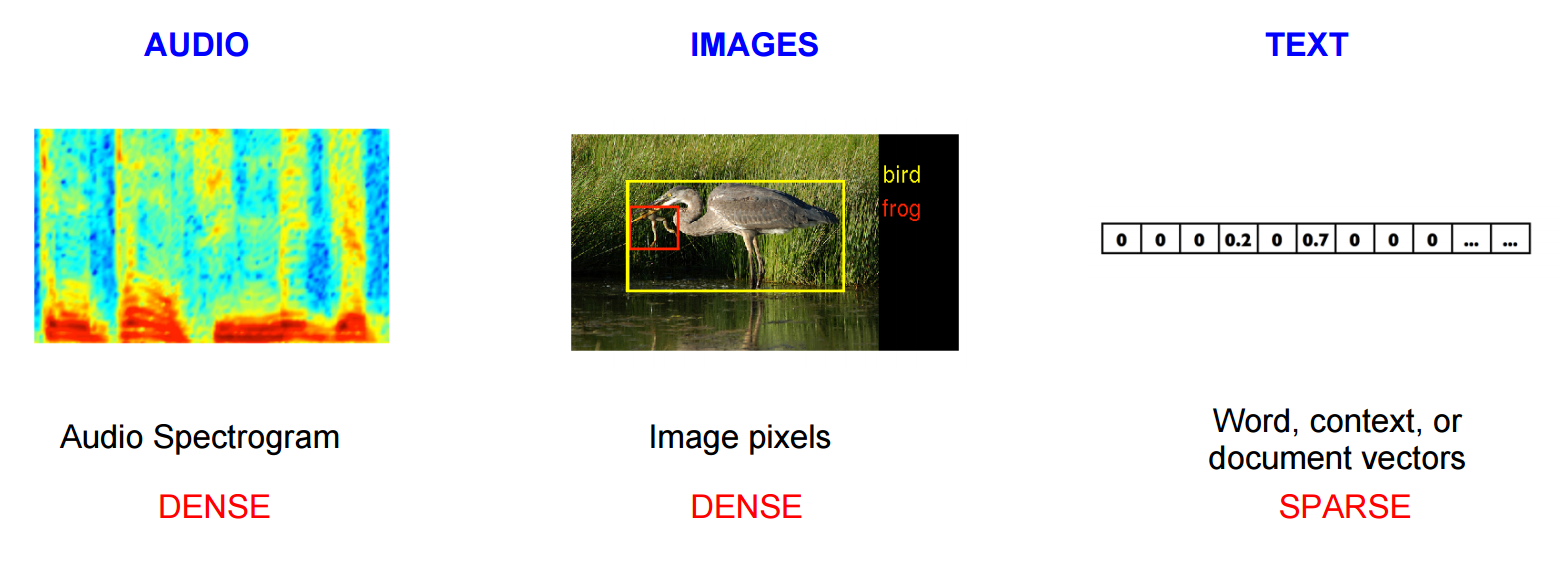
\includegraphics[width=1\textwidth]{images/amira/audio-image-text.png}%
     % you need to add the caption for the list of figures
    \caption[Audio-image-text representation]{audio-image-text image}\label{fig:audio-image-text}%
 \end{figure}
 
\subsection{Vector space models of language words(VSMs)}
    VSMs represent (embed) words in a continuous vector space where semantically similar words are mapped to nearby points ('are embedded nearby each other').
    VSMs have a long, rich history in NLP, but all methods depend in some way or another on the Distributional Hypothesis, which states that words that appear in the same contexts share semantic meaning. The different approaches that leverage this principle can be divided into two categories:
  
 \begin{enumerate}
      \item\textcite{Count-based methods} \\
          Count-based methods (e.g. Latent Semantic Analysis) compute the statistics of how often some word co-occurs with its neighbor words in a large text corpus, and then map these count-statistics down to a small, dense vector for each word.
      \item\textcite{predictive methods} \\
            Predictive models (e.g. neural probabilistic language models) directly try to predict a word from its neighbors in terms of learned small, dense embedding vectors (considered parameters of the model).
      
  \end{enumerate}
  
\subsection{Word2vec}
  Word2vec is a particularly computationally-efficient predictive model for learning word embeddings from raw text. It comes in two flavors:
  \begin{enumerate}
      \item\textcite{ Continuous Bag-of-Words model}(CBOW)\\
            The first proposed architecture is similar to the feedforward NNLM, where the non-linear hidden layer is removed and the projection layer is shared for all words (not just the projection matrix). thus, all words get projected into the
            same position (their vectors are averaged). We call this architecture a bag-of-words model as the order of words in the history does not influence the projection. Furthermore, we also use words from the future; we have obtained the best performance on the task introduced in the next section by building a log-linear classifier with four future and four history words at the input, where the training criterion is to correctly classify the current (middle) word.
            We denote this model further as CBOW, as unlike standard bag-of-words model, it uses continuous distributed representation of the context. The model architecture is shown at Figure 3.2. Note that the weight matrix between the input and the projection layer is shared for all word positions in the same way as in the NNLM \cite{DBLP:journals/corr/abs-1301-3781}.
  
     \item\textcite{Skip-Gram model}\\
            The second architecture is similar to CBOW, but instead of predicting the current word based on the context, it tries to maximize classification of a word based on another word in the same sentence. More precisely, we use each current word as an input to a log-linear classifier with continuous projection layer, and predict words within a certain range before and after the current word. We found that increasing the range improves quality of the resulting word vectors, but it also increases the computational complexity. Since the more distant words are usually less related to the current word than those close to it, we give less weight to the distant words by sampling less from those words in our training examples \cite{DBLP:journals/corr/abs-1301-3781}.
  \end{enumerate}
  
This inversion might seem like an arbitrary choice, but statistically it has the effect that CBOW smoothes over a lot of the distributional information (by treating an entire context as one observation). For the most part, this turns out to be a useful thing for smaller datasets. However, skip-gram treats each context-target pair as a new observation, and this tends to do better when we have larger datasets. We will focus on skip-gram model.

 \begin{figure}[H]%
     \center%
     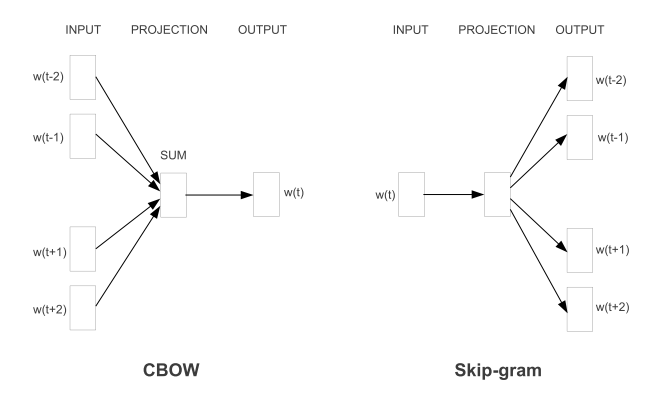
\includegraphics[width=0.8\textwidth]{images/amira/cbow+skip.PNG}%
      % you need to add the caption for the list of figures
     \caption[CBOW and Skip-gram models architecture]{New model architectures. The CBOW architecture predicts the current word based on the context, and the Skip-gram predicts surrounding words given the current word.}\label{fig:cbow}%
 \end{figure}
 
\subsubsection{Scaling up with Noise-Contrastive Training}
     Neural probabilistic language models are traditionally trained using the \textbf{maximum likelihood} (ML) principle to maximize the probability of the next word ${w_t}$(for "target") given the previous words ${h}$  (for "history") in terms of a softmax function\cite{web001}\@.

 \begin{equation}
       \large
          P(w_t | h) = \text{softmax} (\text{score} (w_t, h)) \\
                     = \frac{\exp \{ \text{score} (w_t, h) \} }
                     {\sum_\text{Word w' in Vocab} \exp \{ \text{score} (w', h) \} }
 \end{equation}
 
where \text score({$w_t$}, $h$) computes the compatibility of word ${w_t}$ with the context ${h}$ (a dot product is commonly used). We train this model by maximizing its log-likelihood on the training set, i.e. by maximizing. 
 \begin{equation}
        \large 
           J_\text{ML} = \log P(w_t | h)
                       = \text{score} (w_t, h) -
                       \log \left( \sum_\text{Word w' in Vocab} \exp\{ \text{score} (w', h) \} \right)
 \end{equation}
 This yields a properly normalized probabilistic model for language modeling. However this is very expensive, because we need to compute and normalize each probability using the score for all other $V$  words $w'$ in the current context $h$ , at every training step.
\begin{figure}[H]%
    \center%
    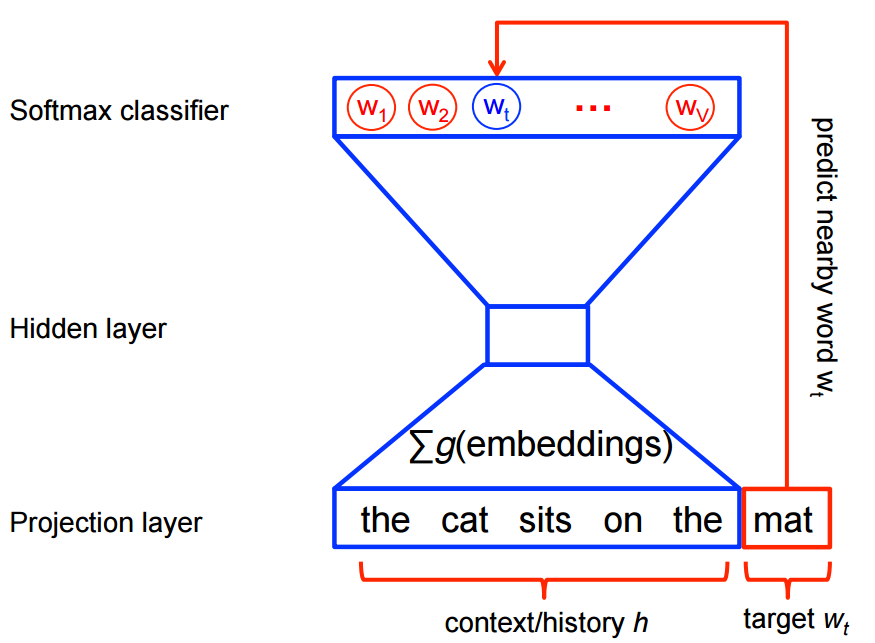
\includegraphics[width=0.6\textwidth]{images/amira/softmax-nplm.png}%
    % you need to add the caption for the list of figures
    \caption[Word2vec architecture]{softmax-nplm}\label{fig:softmax}%
  \end{figure}
  

\subsubsection{Negative Sampling}
On the other hand, for feature learning in word2vec we do not need a full probabilistic model. The CBOW and skip-gram models are instead trained using a binary classification objective (logistic regression) to discriminate the real target words $w_t$ from $k$ imaginary (noise) words $\tilde w$, in the same context..For skip-gram the direction is simply inverted.\\ Mathematically, the objective (for each example) is to maximize:
  \begin{equation}
     \large
        J_\text{NEG} = \log Q_\theta(D=1 |w_t, h) +
        k {\space{E}}_{\tilde w \sim P_\text{noise}}
        \left[ \log Q_\theta(D = 0 |\tilde w, h) \right]
  \end{equation}
  where $Q_\theta(D=1 | w, h)$  is the binary logistic regression probability under the model of seeing the word $w$ in the context $h$ in the dataset $D$ , calculated in terms of the learned embedding vectors $\theta$ . In practice we approximate the expectation by drawing $k$  contrastive words from the noise distribution.

 This objective is maximized when the model assigns high probabilities to the real words, and low probabilities to noise words. Technically, this is called \textcite{ Negative Sampling}, and there is good mathematical motivation for using this loss function: The updates it proposes approximate the updates of the softmax function in the limit. But computationally it is especially appealing because computing the loss function now scales only with the number of noise words that we select ($k$), and not all words in the vocabulary ($V$). This makes it much faster to train.
 
\subsubsection{Noise-Contrastive Estimation}

We will actually make use of the very similar Noise-Contrastive Estimation (NCE) loss. NCE posits that a good model should be able to differentiate data from noise by means of logistic regression. While NCE can be shown to approximately maximize the log probability of the softmax, the Skip-gram model is only concerned with learning high-quality vector representations, so we are free to simplify NCE as long as the vector representations retain their quality \cite{DBLP:journals/corr/MikolovSCCD13}.

\begin{figure}[H]%
    \center%
    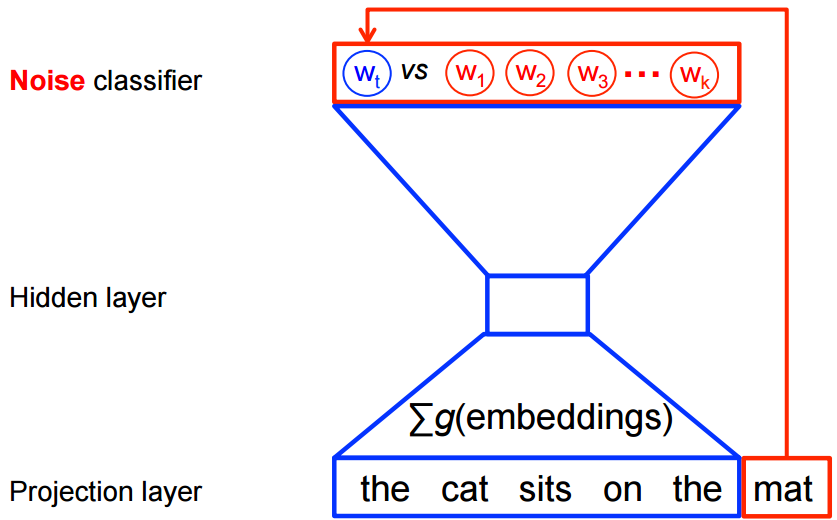
\includegraphics[width=0.6\textwidth]{images/amira/nce-nplm.png}%
    % you need to add the caption for the list of figures
    \caption[Negative Sampling Graph]{nce-nplm}\label{fig:nce-nplm}%
\end{figure}

The main difference between the Negative sampling and NCE is that NCE needs both
samples and the numerical probabilities of the noise distribution, while Negative sampling uses only samples. And while NCE approximately maximizes the log probability of the softmax, this property is not important for our application \cite{DBLP:journals/corr/MikolovSCCD13}.
\subsubsection{Visualization}
\label{visual}
 We can visualize the learned vectors by projecting them down to 2 dimensions using for instance something like the \textcite{t-SNE dimensionality reduction technique}.\\ When we inspect these visualizations it becomes apparent that the vectors capture some general, and in fact quite useful, semantic information about words and their relationships to one another. It was very interesting when we first discovered that certain directions in the induced vector space specialize towards certain semantic relationships, e.g. male-female, verb tense and even country-capital relationships between words, as illustrated in the figure below:
 
  \begin{figure}[H]%
      \center%
        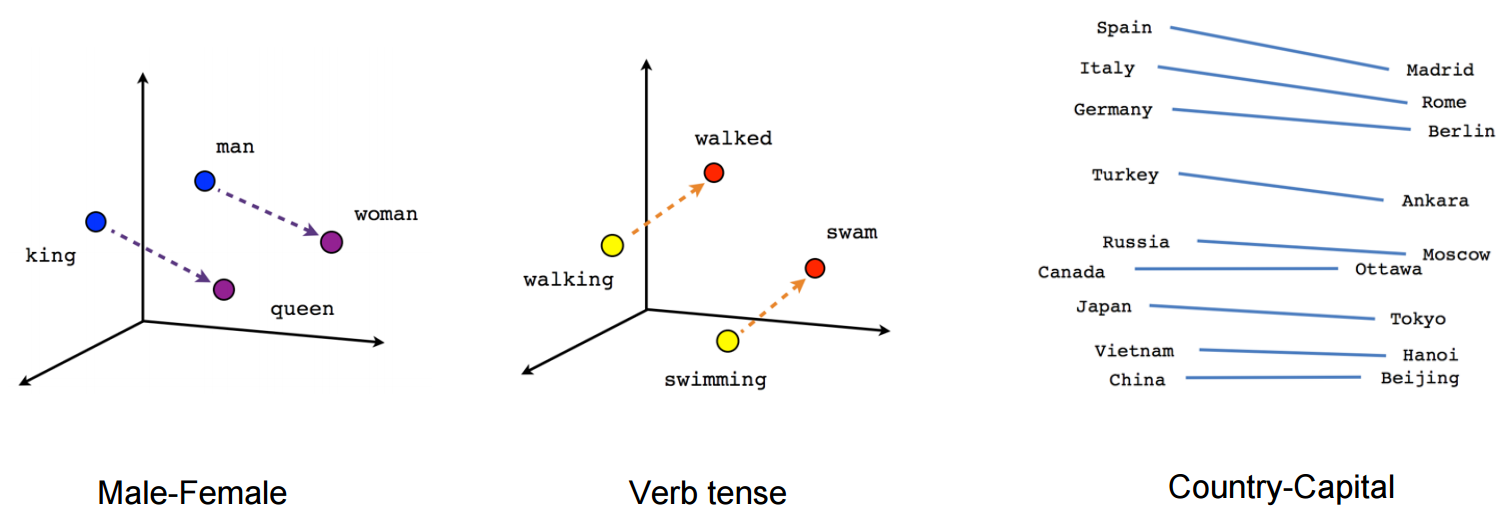
\includegraphics[width=1\textwidth]{images/amira/linear-relationships.png}%
        % you need to add the caption for the list of figures
        \caption[Analogies between words]{linear relationships}\label{fig:nce-nplm}%
  \end{figure}


\subsection{Glove: Global Vectors for Word Representation}
These real-valued word vectors have proven to be useful for all sorts of natural language processing tasks, including parsing, named entity recognition, and (very recently!) machine translation\cite{pennington2014glove}.
It’s been shown (and widely shared by this point) that these word vectors exhibit interesting semantic and syntactic regularities. For example, we find that claims like the following hold for the associated word vectors:
 \begin{align*}\text{king} - \text{man} + \text{woman} &\approx \text{queen} \\ \text{brought} - \text{bring} + \text{seek} &\approx \text{sought}\end{align*}
 The GloVe model learns word vectors by examining word co-occurrences within a text corpus. Before we train the actual model, we need to construct a co-occurrence matrix $X$, where a cell $X_{ij}$ is a “strength” which represents how often the word $i$ appears in the context of the word $j$. We run through our corpus just once to build the matrix $X$, and from then on use this co-occurrence data in place of the actual corpus. We will construct our model based only on the values collected in $X$.
Once we’ve prepared $X$, our task is to decide vector values in continuous space for each word we observe in the corpus. We will produce vectors with a soft constraint that for each word pair of word $i$ and word $j$.

 \begin{equation}
     \vec{w}_i^T \vec{w}_j + b_i + b_j = \log X_{ij}
 \end{equation}
 
where $b_i$ and $b_j$ are scalar bias terms associated with words $i$ and $j$, respectively. Intuitively speaking, we want to build word vectors that retain some useful information about how every pair of words $i$ and $j$ co-occur.
We’ll do this by minimizing an objective function J, which evaluates the sum of all squared errors based on the above equation, weighted with a function $f$:
\begin{equation}
\large
J = \sum_{i=1}^V \sum_{j=1}^V \; f\left(X_{ij}\right) \left( \vec{w}_i^T \vec{w}_j + b_i + b_j - \log X_{ij} \right)^2 
\end{equation}

We choose an $f$ that helps prevents common word pairs (i.e., those with large $X_{ij}$ values) from skewing our objective too much:
 \begin{equation}
     \large
      f\left(X_{ij}\right) = \left\{ \begin{array}{cl}\left(\frac{X_{ij}}{x_{\text{max}}}\right)^\alpha 
      & \text{if } X_{ij} < x_{\text{max}} \\ 1 & \text{otherwise.} \end{array}\right. \end{equation}
      
When we encounter extremely common word pairs (where $X_{ij}>{x_{max}}$) this function will cut off its normal output and simply return $1$. For all other word pairs, we return some weight in the range $(0,1)$ , where the distribution of weights in this range is decided by $\alpha$.
\subsubsection{Visualization}
Similar to word2vec visualization \ref{visual}.
\subsection{Latest research highlights in word representation}
It is easy to be amazed by their seemingly magical power of word2vec. But in real business use cases, we rarely need to understand single words. So, concentration on recent advances in word vector representation  becomes very important today and some of these improvements are:
\begin{itemize}
    \item Word sense
    \item As guassian clouds
       \begin{itemize}
              \item word2vec as a sort of variation autoencoder
       \end{itemize}
    \item Sub-word information
        \begin{itemize}
              \item in the word anti disestablishmentarianism the ngrams.
              \item anti,dis,ment,rian and ism contain meaning, even if you have not seen the word before.
       \end{itemize}
    \item Context vectors
       \begin{itemize}
             \item helps deal with wordsense
      \end{itemize}
\end{itemize}
 Currently, There are other state-of-the-art word embedding methods which achieve these improvements and used today in Business. Some of these word embedding methods created by Google, Facebook, ..etc:
 \begin{itemize}
     \item \textbf{fastText}\\
     learning is very fast! in order to consider morphemes, each word is represented by the character ngram and vector expressions of them is learned\cite{web004}.
     \item \textbf{Eigenword}\\
     is an real-valued vector "embedding" associated with a word that captures its meaning in the sense that distributionally similar words have similar eigenwords.
     
     \item  \textbf{Dependency-Based Word Embeddings}\\
      by learning dependency-based contexts, it became strong against syntactic similarity. it might be good if you want to use it for syntactic similarity\cite{levy2014dependencybased}.
      
      \item \textbf{ Meta-embedding}\\
     by combining different public embedding sets, better vectors(meta-embeddings) are generated\cite{DBLP:conf/acl/YinS16}.
 \end{itemize} 